%!TEX root = ../main.tex

\chapter{FFTbor}
\label{ch:fftbor}

\lhead{FFTbor: Coarse-Grained Energy Landscapes}

\section{Introduction}
\label{sec:fftbor:intro}

In this chapter, we present the \fftbor algorithm and accompanying software.
\fftbor is a novel algorithm developed with the intent of efficiently computing
the Boltzmann probability of those structures which, for a given input RNA
sequence \seq, differ by $k$ base pairs. By leveraging polynomial interpolation
via the \fft, this algorithm runs in \On{4} time and
\On{2} space, a significant improvement over its predecessor. The accompanying
software which implements this algorithm has been used to evaluate the
correlation between kinetic folding speed and landscape ruggedness.

\subsection{Organization}
\label{subsec:fftbor:org}

This chapter is organized in the following fashion. First, we provide
background on
the problem which \fftbor aims to address, as well as a brief overview of
existing approaches. We follow by a formal explanation of the problem, and
proceed to describe how the energy landscape is coarsified into discrete bins.
We then develop the recursions for the parameterized partition function using
the Nussinov-Jacobson energy model, which allows us to highlight the novel aspects
of the algorithm. After developing the recursions, we indicate how they can be
reformulated as a polynomial whose coefficients $z_k=\bfZ{k}{1,n}$. We then
describe how the \fft can be employed to efficiently compute the coefficients
$z_k$, finishing our description of the underlying algorithm. Then we proceed
to present an application of \fftbor, in the area of RNA folding kinetics.

\section{Background}
\label{sec:fftbor:bkgrnd}

In \citep{freyhult.b07}, a dynamic programming algorithm
\rnabor---pronounced {\em RNA neighbor}---was developed which simultaneously
computes for
each integer $k$, the Boltzmann probability $\pk = \frac{\bfZ{k}{}}{\fullZ}$
of the subensemble of structures
whose \bpd to a given {\em initial}, or
{\em reference}, structure \strSt is $k$.
\footnote{As later
explained, \fullZ denotes the partition function, defined as the sum of
all Boltzmann factors \boltzf{\str}, over all secondary structures \str
of a given RNA sequence, and $R$ denotes the universal
gas constant and $T$ absolute temperature. Similarly \bfZ{k}{} denotes the
sum of all Boltzmann factors of all structures \str, whose \bpd
to the initial structure \strSt is exactly $k$.}
\rnabor stores the value of the (partial)
partition functions \bfZ{k}{i,j} for all $1 \leq i \leq j \leq n$ and
$0 \leq k \leq n$, each of which requires quadratic time to compute.
Thus it follows that \rnabor runs in time \On{5} and space
\On{3}, which severely limits its applicability to genomic annotation.
This restriction is somewhat mitigated by the fact that
in \citep{cloteloulorenz}, we showed how to use sampling
\citep{ding.nar03} to efficiently approximate
\rnabor in cubic time \On{3} and quadratic space \On{2},
{\em provided} that the starting structure \strSt is the \mfe
(MFE) structure. We expect that a more efficient version of
\rnabor could be used in applications in genomics and synthetic
biology, to detect potential conformational switches---
RNA sequences containing two or more (distinct) metastable structures.

In this chapter, we describe a radically different algorithm, \fftbor
\citep{senter.po12},
prounounced {\em FFT neighbor},
that uses polynomial interpolation to compute the
coefficients $p_0,\ldots,p_{n-1}$ of the polynomial defined in
\eqnref{fftbor:pOfX},
where \pk is defined by $\pk = \frac{\bfZ{k}{}}{\fullZ}$.
Due to severe numerical instability issues in both the Lagrange
interpolation formula and in Gaussian elimination, we employ
the \fft (FFT) to compute the \idft (DFT) on values $y_0,\ldots,y_{n-1}$,
where $y_k = p(\omega^k)$ and
$\omega = \pRoU$ is the principal \nRoU and
$p(x)$ is defined in \eqnref{fftbor:pOfX}. This
gives rise to an improved version of \rnabor, denoted \fftbor,
which runs in time \On{4} and space \On{2}.
% Once two metastable structures \strST are identified, we can
% subsequently evaluate the feasibility of transition between
% structures \strS and \strT,
% by computing the {\em barrier energy} using algorithms, such as that
% described in Dotu et al. \citep{dotu.nar10} or Flamm et al.
% \citep{flamm.r01}.

\section{Formalization of the problem}
\label{sec:fftbor:formal}

\fftbor aims to compute the coefficients $p_0,\dots,p_{n-1}$ of the polynomial

\begin{align}
\label{eq:fftbor:pOfX}
p(x) = p_0 + p_1 x + p_2 x^2 + \dots + p_{n-1} x^{n-1},
\end{align}

where \pk is defined as $\pk = \frac{\bfZ{k}{}}{\fullZ}$. We employ the \fft to compute
the \idft on values $y_0,\dots,y_{n-1}$, where
$y_k = p(\omega^k)$ and $\omega = \pRoU$ is the principal \nRoU and $p(x)$ is defined in
\eqnref{fftbor:pOfX}. By leveraging
\nRoUs in conjunction with the \idft the we subvert numeric instability
issues observed with both Lagrange interpolation and Gaussian elimination.

Consider an RNA sequence $\seq = \seqN$, where
$s_i \in \{\text{A,\,U,\,G,\,C}\}$, i.e. a sequence of nucleotides. We can describe a
secondary structure \str which is compatible with \seq as a collection of
base pair tuples $(i,j)$, where $1 \le i \le i+\theta < j \le n$ and
$\theta \ge 0$ (generally taken to be 3), the minimum number of unpaired bases
in a hairpin loop due to steric constraints.

To more simply develop the underlying recursions for \fftbor, we introduce a
number of constraints on the base pairs within \str. Firstly, we require that
each base pair is either a Watson-Crick or G-U wobble, i.e. base pair $(i,j)$
for sequence \seq has corresponding nucleotides $(s_i,s_j)$, which are
restricted to the set

\begin{align}
\label{eq:fftbor:validBP}
\bpSet =
\{\text{(A,\,U),\,(U,\,A),\,(G,\,C),\,(C,\,G),\,(G,\,U),\,(U,\,G)}\}.
\end{align}

With
this constraint satisfied we say that \str is {\em compatible} with \seq, and
for the remainder of this chapter will only consider those structures which are
compatible with \seq.
Secondly, we insist that given two base pairs $(i,j), (x,y)$ from \str,
$i=x \iff j=y$ (bases have at most one partner). Finally, we require that
$i<x<j \iff i<y<j$ (no pseudoknots are allowed). While pseudoknots have been
shown to be present in some biologically relevant RNAs, their inclusion greatly
complicates the recursive decomposition of the structure, and thus it is common
to ignore them.

Provided two secondary structures \strST, we can define a notion of
distance between them. There are a number of different definitions of distance
used across the literature; we will use {\em \bpd} for \fftbor.
\Bpd is defined as the symmetric difference between the sets
\strST:

\begin{align}
\label{eq:fftbor:dBP}
\dBP{\str}{\strT} = |\str \cup \strT| - |\str \cap \strT|.
\end{align}

Given this definition of distance, two structures \str and \strT are said to
be \kNbrs if $\dBP{\str}{\strT} = k$. It is important to note that
the notion of \bpd is also applicable to restrictions of secondary structures
on the subsequence $\seq_{i,j}$,
i.e. $\str_{[i,j]} = \{ (x,y) \,:\, i \leq  x < y \leq j,  (x,y) \in \str \}$.

For a restriction of base pairs for a given structure $\str_{[i,j]}$,
$\strT_{[i,j]}$ is said to be a \kNbr of $\str_{[i,j]}$ if

\begin{align}
\label{eq:fftbor:dBPonRestriction}
\dBP{\str_{[i,j]}}{\strT_{[i,j]}} =
|\{ (x,y): i \leq x<y\leq j,
(x,y) \in \str - \strT \text{or} (x,y) \in \strT - \str \}| = k.
\end{align}

\section{Derivation of the \fftbor algorithm}
\label{sec:fftbor:math}

Given an RNA sequence $\seq=\seqN$ and compatible secondary structure
\strSt, let \bfZ{k}{} denote the sum of the Boltzmann factors
\boltzf{\str} of all \kNbrs \str of \strSt; i.e.

\begin{align}
\bfZ{k}{} = \bfZ{k}{1,n} =
\sum_{\mathclap{\substack{\str \text{ such that } \rule[-.5ex]{0pt}{0pt} \\
 \dBP{\str}{\strSt}=k}}}\;
\boltzF{\str}
\end{align}

where $E(\str)$ denotes the Turner (nearest neighbor)
energy \citep{}
of \str, $R = 0.00198$ kcal/mol denotes the universal
gas constant and $T$ denotes absolute temperature. From this, it follows that
the full partition function is defined as

\begin{align}
\label{eq:fftbor:partFunc}
\fullZ = \bfZ{}{1,n} = \sum_{k=0}^n \bfZ{k}{1,n}
\end{align}

since the \bpd between \strSt and \str is at most

\begin{align}
\label{eq:fftbor:maxDist}
\dBP{\strSt}{\str} \leq |\strSt| + \lfloor \frac{n-\theta}{2} \rfloor \leq n.
\end{align}

We can then define the Boltzmann probability of all \kNbrs of \strSt as

\begin{align}
\label{eq:fftbor:probK}
p(k) =\frac{\bfZ{k}{1,n}}{\bfZ{}{1,n}}.
\end{align}

By visualizing the probabilities \pk as a function of $k$, we generate a
coarse-grained view of the one-dimensional energy landscape of \seq with
respect to \strSt. When \strSt is taken to be the \mfes for example, one would
anticipate to see a peak at $k=0$, with additional peaks implying additional
metastable structures; local energy minima which could suggest an energetic
trap while folding.

\subsection{Definition of the partition function
\texorpdfstring{\bfZ{k}{1,n}}{}}
\label{subsec:fftbor:recursions}

For the rest of the chapter, we consider both \seq as well as the
secondary structure \strSt on \seq to be fixed. We now recall the
recursions from Freyhult et al. \citep{Freyhult.ab05} to determine
the partition function \bfZ{k}{i,j} with
respect to the Nussinov-Jacobson
energy $E_0$ model \citep{nussinovjacobson}, defined by
$-1$ times the number of base pairs; i.e. $E_0(S) = -1 \cdot |S|$.
Although we describe here the recursions for the Nussinov-Jacobson
model, for the sake of
simplicity of exposition, both \rnabor
\citep{Freyhult.ab05} as well as our current software \fftbor,
concern the Turner energy model (described in \Secref{sec:fftbor:turner}), consisting of free energy parameters for
stacked bases, hairpins, bulges, internal loops and multiloops.

% The full
% recursions for \fftbor are described for the
% the Turner energy model in the appendix.

The base case for \bfZ{k}{i,j} is given by

\begin{align}
\label{eq:fftbor:initZpart1}
\bfZ{0}{i,j} = 1, \text{ for } i \le j,
\end{align}

since the only 0-neighbor to a structure \strSt
is the structure \strSt itself, and

\begin{align}
\label{eq:fftbor:initZpart2}
\bfZ{k}{i,j} = 0, \text{ for } k > 0, i \le j \leq i + \theta,
\end{align}

since the empty structure is the only possible structure for a
sequence shorter than $\theta + 2$ nucleotides, and so there are no
\kNbrs for $k>0$. The recursion used to compute
\bfZ{k}{i,j} for $k > 0$ and $j > i+\theta$ is

\begin{align}
\label{eq:fftbor:bfZkij}
\bfZ{k}{i,j} = \bfZ{k-b_0}{i,j-1}\enspace +
\sum_{\substack{(s_r,s_j) \in \bpSet, \\ i \leq r<j}}\qquad
\sum_{\mathclap{w+w'=k-b(r)}}\enspace
\exp(-E_0(r,j)/RT) \cdot \bfZ{w}{i,r-1} \bfZ{w'}{r+1,j-1},
\end{align}

where $E_0(r,j) = -1$ if positions $r,j$ can pair in sequence \seq,
and otherwise $E_0(r,j) = +\infty$. Additionally,
$b_0 = 1$ if $j$ is base-paired
in $\strSt_{[i,j]}$ and $0$ otherwise, and
$b(r)=\dBP{\strSt_{[i,j]}}{\strSt_{[i,r-1]} \cup \strSt_{[r+1,j-1]} \cup\{(r,j)\}}$.
This holds since in a secondary
structure $\strT_{[i,j]}$ on \seqIJ that is a \kNbr of
$\strSt_{[i,j]}$,
either nucleotide $j$ is unpaired in $[i,j]$ or it is
paired to a nucleotide $r$ such that $i \leq r < j$. In this
latter case it is enough to study the smaller sequence segments
$[i,r-1]$ and $[r+1,j-1]$ noting that, except for $(r,j)$,
base pairs outside of these regions are not allowed, since there
are no pseudoknots. In addition,
for $\dBP{\strSt_{[i,j]}}{\strT_{[i,j]}} = k$ to hold,
it is necessary for $w+w' = k -b(r)$ to hold, where $w =
\dBP{\strSt_{[i,r-1]}}{\strT_{[i,r-1]}}$ and $w' =
\dBP{\strSt_{[r+1,j-1]}}{\strT_{[r+1,j-1]}}$, since $b(r)$ is the
number of base pairs that differ between $\strSt_{[i,j]}$ and a
structure $\strT_{[i,j]}$, due to the introduction of the base pair
$(r,j)$.

Given RNA sequence \seq and compatible initial structure \strSt,
we define the {\em polynomial}

\begin{align}
\label{eq:fftbor:zOfX}
\fullZx = \sum_{k=0}^n z_k x^k
\end{align}

where coefficients $z_k=\bfZ{k}{1,n}$. Moreover, because of
\eqnref{fftbor:maxDist} and the fact that the minimum number of
unpaired bases in a hairpin loop $\theta$ is 3, we know that $z_n=0$,
so that \fullZx is a polynomial of degree strictly less than $n$.
If we evaluate the polynomial \fullZx for $n$ distinct values

\begin{align}
\label{eq:fftbor:solutionsForAlpha}
\emZof{}{a_1} = y_1, \dots, \emZof{}{a_n} = y_n,
\end{align}

then the Lagrange polynomial interpolation formula guarantees that
$\fullZx = \sum_{k=1}^n y_k P_k(x)$, where the polynomials $P_k(x)$ have degree
at most $n-1$ and are given by the Lagrange formula

\begin{align}
\label{eq:fftbor:lagrangeInterpolation}
P_k(x) = \frac{\prod_{i\ne k} (x-x_i)}{\prod_{i \ne k} (x_k-x_i)}.
\end{align}

Since the polynomials $P_k(x)$ can be explicitly computed, it follows that
we can compute the coefficients $z_k$ of polynomial \fullZx. As we describe
below, the evaluation of \fullZx for a fixed value of $x$ can be done in
time \On{3} and space \On{2}.  It follows that the coefficients
$z_k=\bfZ{k}{1,n}$ can be computed after
$n$ evaluations of \fullZx, where the space for each evaluation of \fullZx
is re-used; hence these evaluations can be performed in time \On{4} and space
\On{2}. Finally,
Lagrange interpolation is clearly computable in time \On{3}.
Although this approach is theoretically sound, there are severe
numerical stability issues related to the interpolation method
\citep{highambarycentricinterpolation},
the choice of values $a_1,\dots,a_{n}$ in the interpolation,
and floating point arithmetic (round-off error) related to the
astronomically large values of the partition functions
\bfZ{k}{1,n}, for $0 \leq k < n$. After many unsuccessful
approaches including scaling we obtained excellent results by
interpolating the polynomial $p(x)$, defined in \eqnref{fftbor:pOfX},
rather than the polynomial \fullZx, defined in \eqnref{fftbor:zOfX},
and performing interpolation with the \fft (FFT) \citep{cormen}
where \alphaN are
chosen to be \nRoUs,
$\alpha_k = \kRoU$.
One
advantage of the FFT is that interpolation can be performed in $O(n \log n)$
time, rather than the cubic time required by using the Lagrange formula
shown in \eqnref{fftbor:lagrangeInterpolation} or by Gaussian elimination. Fewer
numerical operations implies increased numerical stability in our application.

\subsection{Recursions to compute the polynomial
\texorpdfstring{\emZ{i,j}}{}}
\label{subsec:fftbor:polynomial}

Given an initial secondary structure \strSt of a
given RNA sequence \seq, our goal is to compute

\begin{align}
\label{eq:fftbor:defZofK}
\bfZ{k}{1,n} = \sum_{\mathclap{\substack{\str \text{ such that }\\ \dBP{\str}{\strSt}=k}}}\;
\boltzNuss{\str}
\end{align}

where \str can be any structure compatible with \seq.
As previously mentioned, the recurrence relation for \rnabor
with respect to the Nussinov energy model $E_0$ is

\begin{align}
\label{eq:fftbor:rnaborNuss}
\bfZ{k}{i,j} = \bfZ{k-b_0}{i,j-1}\enspace +
\sum_{\substack{(s_r,s_j) \in \bpSet, \\ i \le r<j}}
\left(
\boltzNuss{r,j}\enspace \sum_{\mathclap{w+w'=k-b(r)}}\quad
\bfZ{w}{i,r-1} \bfZ{w'}{r+1,j-1}
\right)
\end{align}

where $E_0(r,j)=-1$ if $r$ and $j$ can base-pair and otherwise
$+\infty$, and
$b_0 = 1$ if $j$ is base paired in $\strSt_{[i,j]}$ and $0$ otherwise, and
$b(r)=\dBP{\strSt_{[i,j]}}{\strSt_{[i,r-1]} \cup \strSt_{[r+1,j-1]} \cup\{(r,j)\}}$.
The following theorem shows that an analogous recursion can be used to compute
the {\em polynomial} $\emZ{i,j}$ defined by

\begin{align}
\label{eq:fftbor:polynomialZij}
\emZ{i,j} = \sum_{k=0}^n z_k(i,j)\,x^k
\end{align}

where

\begin{align}
z_k(i,j)\>=\>
\bfZ{k}{i,j}\enspace=\enspace
\sum_{\mathclap{\substack{\str \text{ such that } \\
\dBP{\str}{\strSt_{[i,j]}}=k}}}\enspace
\boltzNuss{\str}.
\end{align}

Here, in the summation, \str runs over structures on \seqIJ, which
are \kNbrs of the restriction $\strSt_{[i,j]}$ of initial structure
\strSt to interval $[i,j]$, and
$E_0(S)=-1 \cdot |S|$ denotes the Nussinov-Jacobson energy of \str.

\begin{theorem}
\label{thm:fftbor:recursions}
Let \seqN be a given RNA sequence.
For any integers $1 \leq i \leq j \leq n$, let

\begin{align}
\emZ{i,j} = \sum_{k=0}^n z_k\,x^k
\end{align}

where

\begin{align}
z_k(i,j) = \bfZ{k}{i,j}.
\end{align}

Then for $i\leq j \leq i+\theta$, $\emZ{i,j}=1$ and for
$j>i+\theta$ we have the recurrence relation

\begin{align}
\label{eq:fftbor:fftborNussPoly}
\emZ{i,j} = \emZ{i,j-1} \cdot x^{b_0} +
\sum_{\substack{(s_r,s_j) \in \bpSet, \\ i\le r<j}}
\left(
\boltzNuss{r,j} \cdot \emZ{i,r-1} \cdot \emZ{r+1,j-1} \cdot x^{b(r)}
\right).
\end{align}

where $b_0 = 1$ if $j$ is base-paired in $\strSt_{[i,j]}$ and $0$ otherwise, and
$b(r) =
\dBP{\strSt_{[i,j]}}{\strSt_{[i,r-1]} \cup \strSt_{[r+1,j-1]} \cup \{(r,j)\}}$.
\end{theorem}

\begin{proof}
First, some notation is necessary.
Recall that if $F$ is an arbitrary
polynomial [resp. analytic] function, then $[x^k]F(x)$
denotes the coefficient of $x^k$ [resp. the $k$th Taylor coefficient in the
Taylor expansion of $F(x)$]. For instance, in
\eqnref{fftbor:pOfX}, $[x^k]p(x) = \pk$, and in
\eqnref{fftbor:zOfX}, $[x^k]\fullZx = z_k$.

By definition, it is clear that $\emZ{i,j}=1$ if $i \leq j \leq i + \theta$,
where we recall that $\theta = 3$ is the minimum number of unpaired bases in
a hairpin loop. For $j > i + \theta$, we have

\begin{align}
\begin{split}
[x^k] \emZ{i,j} &= z_k(i,j) = \bfZ{k}{i,j} \\
&= \bfZ{k-b_0}{i,j-1} +
\sum_{r=i}^{j-1}\hspace{2.25em} \sum_{\mathclap{k_0+k_1=k-b(r)}}\hspace{1.5em}
\left( \boltzNuss{r,j} \cdot \bfZ{k_0}{i,r-1} \cdot \bfZ{k_1}{r+1,j-1} \right) \\
&= [x^{k-b_0}] \emZ{i,j-1} \\
&+ \sum_{r=i}^{j-1}\hspace{2.25em} \sum_{\mathclap{k_0+k_1=k-b(r)}}\hspace{1.5em}
\left( \boltzNuss{r,j} \cdot \left( [x^{k_0}] \emZ{i,r-1} \right) \cdot
\left( [x^{k_1}] \emZ{r+1,j-1} \right) \right) \\
&= [x^{k-b_0}] \emZ{i,j-1} \\
&+ \sum_{r=i}^{j-1}\hspace{2.25em} \sum_{\mathclap{k_0+k_1=k-b(r)}}\hspace{1.5em}
\left( \boltzNuss{r,j} \cdot [x^{k_0+k_1}]
\left( \emZ{i,r-1} \cdot \emZ{r+1,j-1} \right) \right).\\
\end{split}
\end{align}

By induction, the proof of the theorem now follows.
\end{proof}

Notice that if one were to compute all terms of the polynomial $\emZ{1,n}$
by explicitly performing polynomial multiplications,
then the computation would require \On{5} time and \On{3} space.
Instead of explicitly performing polynomial expansion in {\em variable} $x$,
we instantiate $x$ to a fixed complex number $\alpha \in \mathbb{C}$, and apply
the following recursion for this instantiation:

\begin{align}
\label{eq:fftbor:fftborNussPolyAlpha}
\emZof{i,j}{\alpha} = \emZof{i,j-1}{\alpha} \cdot \alpha^{b_0} +
\sum_{\substack{(s_r,s_j) \in \bpSet, \\ i \le r<j}}
\left(
\boltzNuss{r,j} \cdot
\emZof{i,r-1}{\alpha} \cdot \emZof{r+1,j-1}{\alpha} \cdot \alpha^{b(r)}
\right).
\end{align}

In this fashion, we can compute $\emZof{}{\alpha}=\emZof{1,n}{\alpha}$ in
\On{3} time and \On{2} space. For $n$ distinct complex values
\alphaN, we can compute and save only the
values $\emZof{}{\alpha_0},\dots,\emZof{}{\alpha_{n-1}}$, each time re-using the
\On{2} space for the next computation of $\emZof{}{\alpha_k}$. It follows that
the computation resources used to determine the (column) vector

\begin{align}
\label{eq:fftbor:yColumn}
\bfY = (y_0,\dots,y_{n-1})^{\text T} =
\left(
\begin{array}{l}
y_0 \\
y_1 \\
\vdots \\
y_{n-1} \\
\end{array}
\right)
\end{align}

where
$y_0=\emZof{}{\alpha_0},\dots,y_{n-1}=\emZof{}{\alpha_{n-1}})$ is thus quartic time \On{4} and quadratic space \On{2}.

\subsection{Polynomial interpolation to evaluate
\texorpdfstring{\emZ{i,j}}{}}
\label{subsec:fftbor:fft}

Let $\omega = \pRoU$ be the principal \nRoU.
Recall that the Vandermonde matrix $V_n$ is defined to be the
$n \times n$ matrix, whose $i,j$ entry is $\omega^{i \cdot j}$; i.e.

\begin{align}
\label{eq:fftbor:vandermonde}
V_n =
\left(
\begin{array}{rrrrr}
1 & 1 & 1 & \dots & 1 \\
1 & \omega & \omega^2 & \dots & \omega^{n-1} \\
1 & \omega^2 & \omega^4 & \dots & \omega^{2(n-1)} \\
1 & \omega^3 & \omega^6 & \dots & \omega^{3(n-1)} \\
\vdots & \vdots & \vdots & \vdots & \vdots \\
1 & \omega^{n-1} & \omega^{2(n-1)} & \dots & \omega^{(n-1)(n-1)} \\
\end{array}
\right)
\end{align}

The \fft is defined to be the $O(n \log n)$
algorithm to compute the Discrete Fourier Transform (DFT), defined
as the matrix product $\bfY = V_n {\bf A}$:

\begin{align}
\label{eq:fftbor:dftMatrix}
\left(
\begin{array}{l}
y_0 \\
y_1 \\
y_2 \\
\vdots \\
y_{n-1} \\
\end{array}
\right)
= V_n \cdot
\left(
\begin{array}{l}
a_0 \\
a_1 \\
a_2 \\
\vdots \\
a_{n-1} \\
\end{array}
\right)
\end{align}

On page $837$ of \citep{cormen}, it is shown that the
$(i,j)$ entry of $V_n^{-1}$ is $\frac{\omega^{-j i}}{n}$
and that

\begin{align}
\label{eq:fftbor:aFromY}
a_j = \frac{1}{n} \sum_{k=0}^{n-1} y_k\,\omega^{-kj}
\end{align}

for $j=0,\dots,n-1$.

Since we defined \bfY in \eqnref{fftbor:yColumn} by $\bfY =
(y_0,\dots,y_{n-1})^{\text T}$, where
$y_0=\emZof{}{\alpha_0},\dots,y_{n-1}=\emZof{}{\alpha_{n-1}})$
and $\alpha_k = \omega^k \kRoU$, it follows that the coefficients
$z_k=\bfZ{k}{1,n}$ in the polynomial
$\fullZx = z_0 + z_1 x + \dots + z_{n-1} x^{n-1}$ defined in
\eqnref{fftbor:zOfX} can be computed, at least in principle,
by using the \fft. It turns out, however, that the values of
\bfZ{k}{1,n} are so astronomically large, that the ensuing numerical
instability makes even this approach infeasible for values of $n$
that exceed $56$ (data not shown).
Nevertheless, our approach can be modified as follows.
Define \bfY by $\bfY = (y_1,\dots,y_n)^{\text T}$, where
$y_1=\frac{\emZof{}{\alpha_1}}{\fullZ},\dots,
y_{n}=\frac{\emZof{}{\alpha_n}}{\fullZ}$, and
\fullZ is the partition function defined in \eqnref{fftbor:partFunc}.
Using the \fft to compute the \idft, it follows from
\eqnref{fftbor:aFromY} that we can compute the probabilities $p_0,\dots,p_{n-1}$
that are coefficients of the polynomial
$p(x) = p_0 + p_1 x + \dots + p_{n-1}x^{n-1}$
defined in \eqnref{fftbor:pOfX}. For genomics applications, we are
only interested in the $m$ most significant digits of each \pk, as described
in the pseudocode on the following page.
\medskip

\begin{figure}[!ht]
\hrule \rule[0ex]{0pt}{0pt}
\begin{center}
{\large Pseudocode for \fftbor} \\
\end{center}
\begin{tabular*}{\textwidth}{ll}
{\sc Purpose:} & Computes the $m$ most significant digits
of probabilities $\pk = \sfrac{\bfZ{k}{1,n}}{\fullZ}$ \rule[-1.5ex]{0pt}{0pt} \\
{\sc Input:} & RNA sequence $\seq = \seqN$, secondary
structure \strSt of \seq, integer $m$ \rule[-1.5ex]{0pt}{0pt} \\
{\sc Output:} & Probabilities $\pk = \sfrac{\bfZ{k}{1,n}}{\fullZ}$ to $m$ significant digits for $k=0,\dots,n-1$ \rule[-1.75em]{0pt}{0pt} \\
\hline \rule[0ex]{0pt}{0pt}
\end{tabular*}
\begin{algorithmic}[1]
\Function{FFTbor}{\seq, \strSt, $m$}
\State $n \gets \textit{length}(\seq)$
\For{$k \gets 0, n-1$}
\Comment{Compute all \nRoUs}
\State $\omega_k \gets \exp(\frac{2 \pi i k}{n})$
\EndFor
\For{$k \gets 0, n-1$}
\Comment{Note that $\emZof{}{\omega_0} = \fullZ$}
\State $y_k \gets 10^m \cdot \frac{\emZof{}{\omega_k}}{\emZof{}{\omega_0}}$
\EndFor
\For{$k \gets 0, n-1$}
\Comment{Compute IDFT from \eqnref{fftbor:aFromY}}
\State $a_k \gets \frac{1}{n} \sum_{j=0}^{n-1} y_j\, \omega^{-kj}$
\State $\pk \gets 10^{-m} \cdot \lfloor a_k \rfloor$
\Comment{Truncate to $m$ significant digits}
\EndFor
\State \textbf{return} $p_0,\dots,p_{n-1}$
\Comment{Return all \pk for $0 \leq k < n$,
from \eqnref{fftbor:probK}}
\EndFunction
\rule[-0.35ex]{0pt}{0pt}
\end{algorithmic}
\caption[Pseudocode for \fftbor]{The function {\sc FFTbor} computes the $m$ most significant digits
of $p_0,\dots,p_{n-1}$, where $\pk = \frac{\bfZ{k}{}}{\fullZ}$. This algorithm
operates in \On{4} time and \On{2} space, a significant improvement over its
predecessor \rnabor.}
\label{fig:fftbor:algo}
\rule[0ex]{0pt}{1.5em} \hrule
\end{figure}

\section{Benchmarking and performance considerations}
\label{sec:fftbor:benchmarking}

In this subsection, we show that we need only evaluate the polynomial
\fullZx, as defined in
\eqnref{fftbor:zOfX}, for $n/2$ of the \nRoUs.
 It is first necessary to recall the definition of complex
conjugate.
Recall that the complex conjugate of $z$ is denoted by $\overline{z}$;
i.e. if $z=\aPbi$ where $a,b \in \mathbb{R}$ are real numbers and
$i = \sqrt{-1}$,  then $\overline{z} = \aMbi$.

\begin{lemma}
\label{lem:fftbor:compconj}

If \fullZx is the complex polynomial defined in
\eqnref{fftbor:zOfX}, then for any \nRoU
 $\alpha$, it is the case that $\emZof{}{\overline{\alpha}} =
\overline{\emZof{}{\alpha}}$. In other words, if $\alpha$ is a \nRoU
 of the form \aPbi, where $a,b \in \mathbb{R}$ and $b>0$, and
if $\emZof{}{\aPbi} = A + Bi$ where $A,B \in \mathbb{R}$, then it is the case that

\begin{align}
\emZof{}{\aMbi} = A - Bi.
\end{align}

\end{lemma}

\begin{proof}
Letting $i = \sqrt{-1}$, if
$\theta = \frac{2 \pi}{n}$, then
$\omega = e^{i \theta} = \cos(\theta) + i \sin(\theta)$
is the principal \nRoU, and
$e^{(0) \cdot i \theta} = 1 = \omega^{0}, \dots ,
e^{(n-1) \cdot i \theta} = \omega^{n-1}$ together
constitute the complete collection of all
\nRoUs---i.e. the $n$ unique solutions of
of the equation $x^n -1 = 0$ over the field $\mathbb{C}$ of complex numbers.
Clearly, for any $1 \leq k < n$,
$e^{-i k \theta} = 1 \cdot e^{-i k \theta} =
e^{2 \pi i} \cdot e^{-i k \theta} = e^{i(2 \pi - k \theta)} =
e^{i(n \theta - k \theta)} = e^{i \theta (n - k)}$.
Moreover, if $\omega^k = e^{i k \theta} = a + b i$ where
$b>0$, then we have $e^{-i k \theta} = \aMbi$. It follows that for any
\nRoU of the form \aPbi, where $b>0$, the number \aMbi
is also an \nRoU.

Recall that $\fullZx = \sum_{k=0}^n z_k x^k$, where
$z_k \in \mathbb{R}$ are real numbers representing the partition function
\bfZ{k}{1,n} over
all secondary structures of a given RNA sequence \seqN,
whose \bpd from initial structure
\strSt is $k$. Thus, in order to prove the lemma, it suffices to show
that for all values $k=0,\dots,n-1$, if \aPbi is a
\nRoU, where $a,b \in \mathbb{R}$
and $b>0$, and if $(\aPbi)^k = C+Di$ where $C,D \in \mathbb{R}$, {\em then}
$(\aMbi)^k = C-Di$. Indeed, we have the following.

\begin{align}
\begin{split}
(\aPbi)^m &= \sum_{k=0}^m \binom{m}{k}\; a^{m-k} \cdot (bi)^k \\
(bi)^k  &=
\begin{cases}
b^k    & \text{if $k \equiv 0 \bmod 4$} \\
i b^k  & \text{if $k \equiv 1 \bmod 4$} \\
-b^k   & \text{if $k \equiv 2 \bmod 4$} \\
-i b^k & \text{if $k \equiv 3 \bmod 4$} \\
\end{cases}
\end{split}
\end{align}

\begin{align}
\begin{split}
(\aMbi)^m &= \sum_{k=0}^m \binom{m}{k}\; a^{m-k} \cdot (-bi)^k \\
(-bi)^k &=
\begin{cases}
b^k   & \text{if $k \equiv 0 \bmod 4$} \\
-ib^k & \text{if $k \equiv 1 \bmod 4$} \\
-b^k  & \text{if $k \equiv 2 \bmod 4$} \\
ib^k  & \text{if $k \equiv 3 \bmod 4$} \\
\end{cases}
\end{split}
\end{align}

It follows that each term of the form
$a^{m-k} \cdot (bi)^k$, for $k=0,\dots,m$, is the complex conjugate of
$a^{m-k} \cdot (-bi)^k$, and thus $(\aPbi)^m$ is the complex conjugate of
$(\aMbi)^m$. Since \emZof{}{\aPbi} is a sum of terms of the form $z_k (\aPbi)^k$,
it follows that \emZof{}{\aMbi} is the complex conjugate of \emZof{}{\aPbi}.
This completes the proof of the lemma.

\end{proof}

Lemma \ref{lem:fftbor:compconj} immediately entails that we need only to evaluate \fullZx on $n/2$
many of the \nRoUs---namely, those of the form
\aPbi, where $b \geq 0$. The remaining values of \fullZx are obtained by
taking conplex conjugates of the first $n/2$ values. This, along with a
precomputation of powers of the \nRoUs, leads to an
enormous performance speed-up in our implementation of \fftbor.

\section{Coarse-grained kinetics with \fftbor}
\label{sec:fftbor:kinetics}

The output of \fftbor, as shown in
\Figref{fftbor:tppDistributions}, is a probability distribution,
where the $x$-axis represents the \bpd from an arbitrary,
but fixed secondary structure \strSt, and the $y$-axis represents the
Boltzmann probability $p(k) = \frac{\bfZ{k}{}}{\fullZ}$ that a secondary structure
has \bpd $k$ from \strSt. Arguably, this probability distribution
is an accurate one-dimensional projection of the rugged, high dimensional energy
landscape near structure \strSt,
of the sort artistically rendered in the well-known
energy landscape depicted in Figure 1 of \citep{wolynes.ptam05}.
A hypothesis behind theoretical work in biomolecular folding theory in
\citep{bryngelson.p95}
is that kinetic folding slows down as the energy landscape becomes more
{\em rugged}. This is borne out in our computational experiments for RNA
using \fftbor, as reported
in \Figref{fftbor:tppDistributions}.

We randomly chose two TPP \rb
aptamers from the seed alignment for
Rfam family RF$00059$. The first sequence has EMBL accession code
BX$842649.1$/$277414$--$277318$ and is comprised of the $97$ nt sequence
\seqsplit{%
  ACCUGACGCUAGGGGUGUUGGUGAAUUCACCGACUGAGAAUAACCCUUU%
  GAACCUGAUAGAGAUAAUGCUCGCGCAGGGAAGCAAGAAUAGAAAGAU%
}, while the second sequence
has EMBL accession code AACY$022101973.1$/$389$--$487$ and is comprised of the $99$
nt sequence
\seqsplit{%
  UAUAAGUCCAAGGGGUGCCAAUUGGCUGAGAUGGUUUUAACCAAUCCCUU%
  UGAACCUGAUCCGGUUAAUACCGGCGUAGGAAUGGAUUUUCUCUACAGC%
}.
Rfam consensus and \mfess for both sequences are
depicted in \Figref{fftbor:tppConsensusAndMfe}.
Despite the fact that there is no sequence homology according to
pairwise BLAST \citep{blast}, this figure clearly demonstrates that
consensus and
\mfess closely resemble each other, and that the
structures of both TPP \rb aptamers are quite similar, with the
exception of the leftmost hairpin loop [resp. multiloop].
The MFE structures differ
from the consensus structures principally by the addition of base pairs not
determined by covariation in the Rfam alignment.
Indeed, if we let $\str_0,\str_1$
denote the Rfam consensus structure [resp. MFE structure] for the $97$ nt
sequence with EMBL accession code BX$842649.1$/$277414$--$277318$, then
$\str_0 \setminus \str_1$ has $4$ base pairs, and $\str_1 \setminus \str_0$
 has $7$
base pairs. If we let $\strT_0,\strT_1$
denote the Rfam consensus structure [resp. MFE structure] for the $99$ nt
sequence with EMBL accession code
AACY$022101973.1$/$389$--$487$, then
$\strT_0 \setminus \strT_1$ has $1$ base pair, and $\strT_1 \setminus \strT_0$ has $5$
base pairs.

\begin{figure}[!ht]
\centering
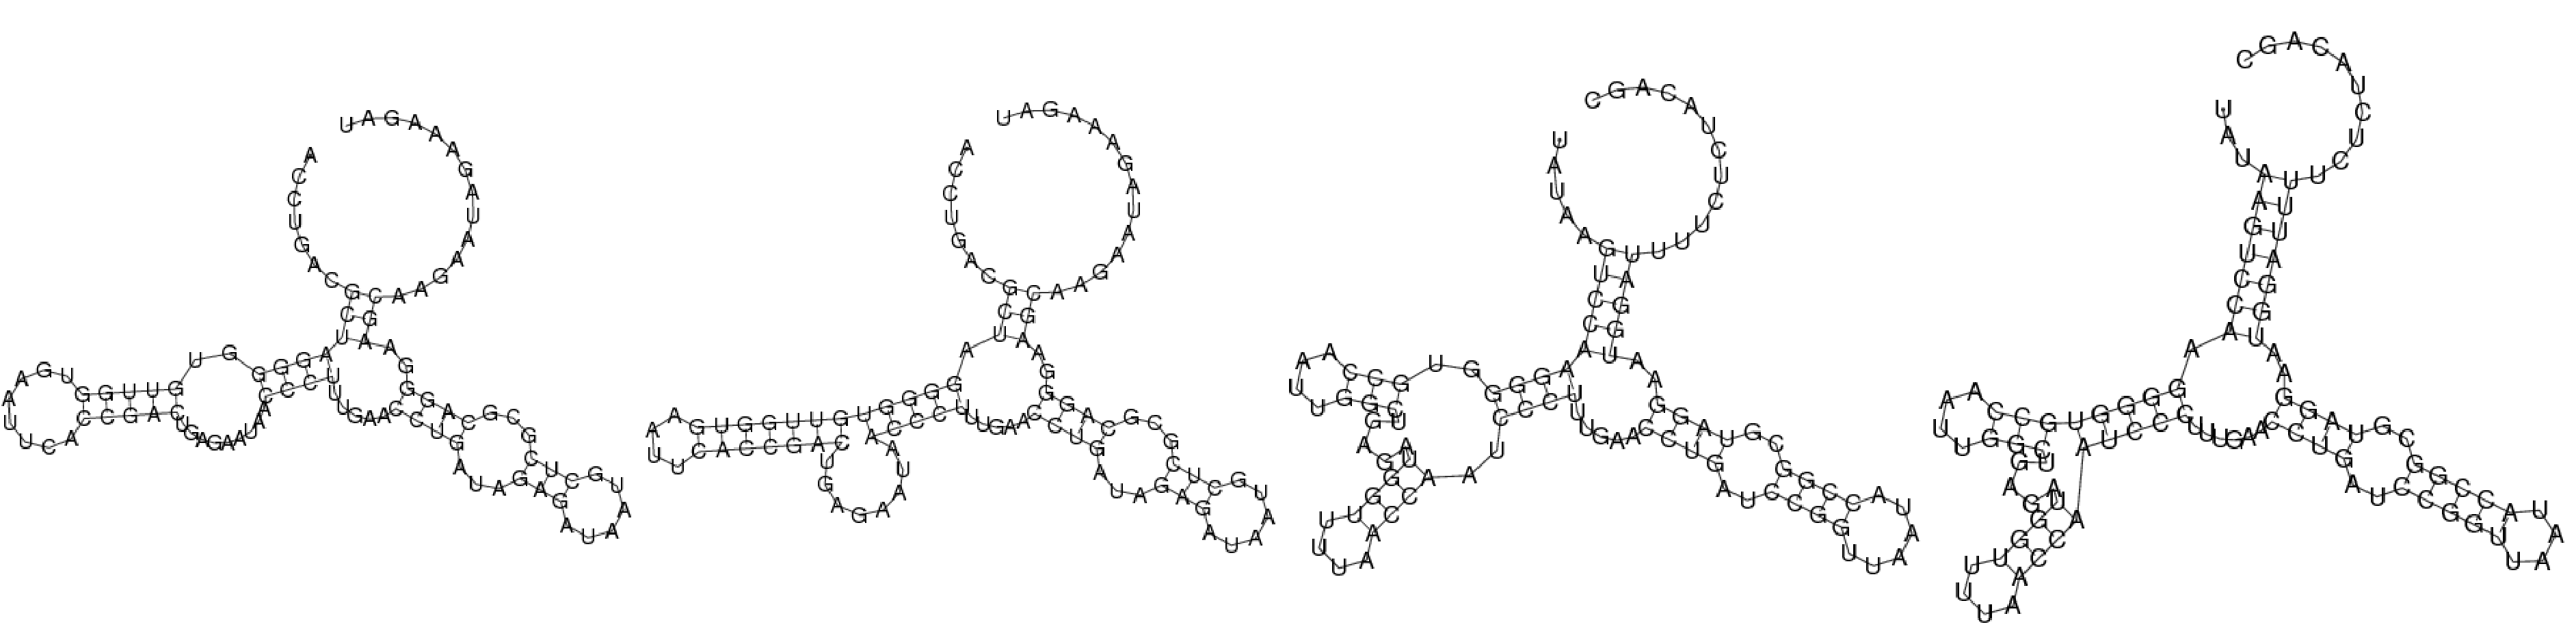
\includegraphics[width=.9\textwidth]{Figures/FFTbor/tppConsensusAndMfe.pdf}
\caption[Rfam consensus structures (Rfam) and \mfe (MFE)
secondary structures for two thiamine pyrophosphate (TPP) \rb aptamers]{Rfam consensus structures (Rfam) and \mfe (MFE)
secondary structures for two thiamine pyrophosphate (TPP) \rb aptamers,
chosen at random from RF$00059$ Rfam family seed alignment
\citep{Gardner.nar11}. Using pairwise BLAST \citep{blast}, there is no
sequence similarity, although the secondary structures are very similar,
as shown in this figure. From left to right:
{\em (A)} MFE structure for BX$842649.1$/$277414$--$277318$.
{\em (B)} Rfam consensus structure for BX$842649.1$/$277414$--$277318$.
{\em (C)} MFE structure for AACY$022101973.1$/$389$--$487$.
{\em (D)} Rfam consensus structure for AACY$022101973.1$/$389$--$487$.
}
\label{fig:fftbor:tppConsensusAndMfe}
\end{figure}

We ran \fftbor on each of the TPP \rb aptamer
sequences, with the MFE structure of each
sequence taken as the initial structure \strSt for that sequence. For the
first sequence, BX$842649.1$/$277414$--$277318$, the \fftbor output
suggests that there are low energy structures
at a distance from the MFE structure, which might compete with the MFE
structure and hence slow the kinetics of folding. In contrast, for the
second sequence, AACY$022101973.1$/$389$--$487$, the \fftbor output suggests
that there are no such competing low energy structures, hence
the second sequence should fold more quickly than the first.

\begin{figure}[!ht]
\centering
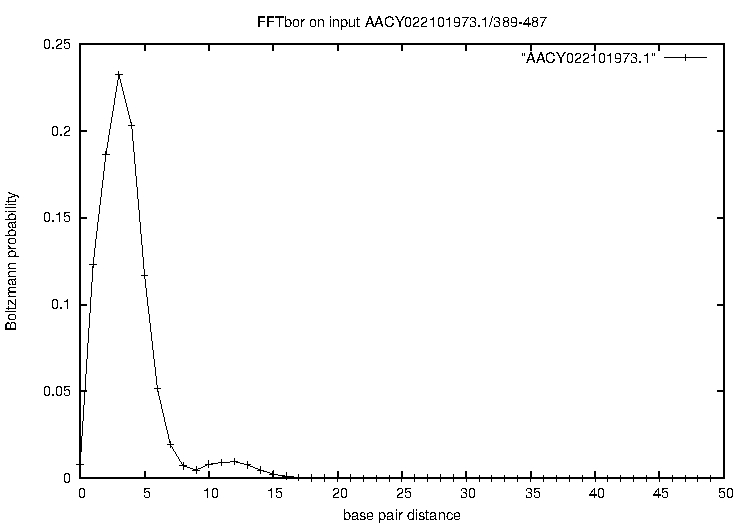
\includegraphics[width=.45\textwidth]{Figures/FFTbor/FFTbor_AACY022101973_1.pdf}
\quad
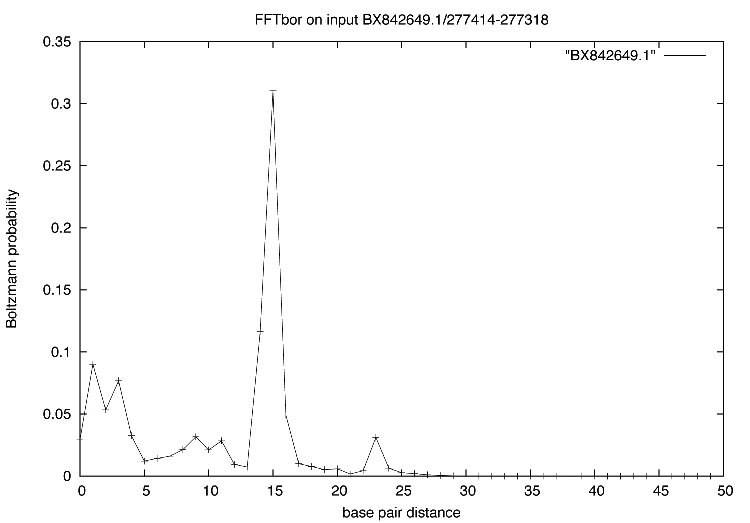
\includegraphics[width=.45\textwidth]{Figures/FFTbor/FFTbor_BX842649_1.pdf}
\caption[Output from \fftbor on two randomly selected
thiamine pyrophosphate \rb (TPP) aptamers]{Output from \fftbor on two randomly selected
thiamine pyrophosphate \rb (TPP) aptamers, taken from the Rfam database
\citep{Gardner.nar11}. The $x$-axis represents \bpd from the
\mfes for each given sequence; the $y$-axis represents
Boltzmann probabilities $p(k) = \sfrac{\bfZ{k}{}}{\fullZ}$, where
\bfZ{k}{} denotes the sum of Boltzmann factors or all secondary structures,
whose \bpd from the MFE structure is exactly $k$.
{\em (Left)}
The $97$ nt sequence BX$842649.1$/$277414$--$277318$ appears to have a rugged energy
landscape near its \mfes, with distinct
low energy structures that may compete with the MFE structure during the
folding process.
{\em (Right)}
The $99$ nt sequence, AACY$022101973.1$/$389$--$487$ appears to have a smooth energy
landscape near its MFE structure, with no distinct low energy structures
to might compete with the MFE structure.
Based on the \fftbor output or {\em structural profile} near MFE
structure \strSt, one might expect
folding time for the first sequence to increase due to competition from
metastable structures, while one might expect the second sequence to have
rapid folding time.
Computational Monte Carlo folding experiments bear out this fact.
\kinfold \citep{flamm} simulations clearly show that the second
sequence folds
at least four times more quickly than the first sequence. See section
\ref{sec:fftbor:kinetics} for
details.}
\label{fig:fftbor:tppDistributions}
\end{figure}

To test the hypothesis that folding is slower for rugged energy landscapes,
we ran the kinetic folding software, \kinfold \citep{flamm},
on each of the two TPP \rb aptamer sequences,
BX$842649.1$/$277414$--$277318$ and AACY$022101973.1$/$389$--$487$,
to determine the \mfpt (MFPT) to
fold into the MFE structure, when starting from the empty structure.
In this computational
experiment, we took MFPT to be the average number of Monte Carlo steps
taken by \kinfold---each step consisting of the addition or removal
of a single base pair---to fold the
empty structure into the MFE
structure, where the average was taken over $30$ runs, with an absolute
maximum number of Monte Carlo steps taken to be $500,000$.
The first sequence, BX$842649.1$/$277414$--$277318$, converged within $500,000$
steps only for $20$ out of $30$ runs. Assigning the maximum step count of
$500,000$ for the $10$ runs that did not converge, we found a \mfpt
of $311,075.06$ steps for this sequence.
The second sequence, AACY$022101973.1$/$389$--$487$, converged within $500,000$
steps in $29$ out of $30$ runs, and we found a \mfpt of
$61,575.69$ steps for this sequence. From computational experiments of this
type, it is suggestive that \fftbor may prove useful in synthetic
biology,
where one would like to design rapidly folding RNA molecules that
fold into a designated target structure.

In order to more systematically determine the relation between kinetic
folding speed and the ruggedness of an energy landscape near the MFE structure,
we need to numerically quantify ruggedness. To this end, in the following
we define the notion of \ebpd to a designated
structure. Let \strSt be an arbitrary secondary structure of the RNA sequence
$\seq = \seqN$.
The expected \bpd to \strSt is defined by

\begin{align}
E[ \{ \dBP{\str}{\strSt} : \str \in \mathbb{S}(\seqN)\} ] =
\sum_{\str} P(\str) \cdot \dBP{\str}{\strSt}
\end{align}

where
$\mathbb{S}(\seqN)$ denotes the set of secondary structures for
$\seq = \seqN$, $P(\str) = \frac{\boltzf{\str}}{\fullZ}$ is the Boltzmann
probability of \str, and
\dBP{\str}{\strSt} denotes \bpd between \str and \strSt.
If we run \fftbor on an input sequence \seq and secondary structure
\strSt, then clearly
$E[ \{ \dBP{\str}{\strSt} : \str \in \mathbb{S}(\seqN)\} ] =
\sum_{k} k \cdot p(k)$, where $p(k)=\frac{\bfZ{k}{}}{\fullZ}$, obtained from the
program output.  If \strSt is the empty structure, then \fftbor output
is simply the probability distribution of the number of base pairs per
secondary structure, taken over the Boltzmann ensemble of all structures.

For the benchmarking assay, we took all $61$ selenocysteine insertion sequence
(SECIS) sequences from the seed alignment of Rfam family RF$00031$
\citep{Gardner.nar11}. Average length was $64.32 \pm 2.83$ nt.
For each sequence, we ran both \fftbor (when starting
from the empty structure rather than the MFE structure) and a Monte Carlo
folding algorithm, developed by E. Freyhult and P. Clote (unpublished).
Using the Monte Carlo algorithm, we
determined the \mfpt (MFPT), defined as the average
taken over $50$ runs, of the number of Monte Carlo steps taken to fold
the empty structure into the MFE structure, where an absolute upper bound
of $5$ million steps was allowed in the simulation.

Surprisingly, we found that there is a significant
correlation of $0.4847$ with one-tailed
$p$-value of $0.0002$ between the
standard deviation of the \fftbor output (when starting from the
empty structure) and logarithm base $10$ of the \mfpt.
As described above, \fftbor output is simply
the probability distribution
for the number of base pairs per structure, taken over the ensemble
of all secondary structure for the input RNA
sequence. The standard deviation of this probability distribution corresponds
to a notion of the {\em width} of the distribution. It is possible that those
sequences having distributions tightly centered around the
mean have faster folding times than those with a wider distribution
due to other local minima causing the RNA to get trapped while folding.

\begin{table}[!ht]
\centering
\begin{tabularx}{\linewidth}{c *{6}{R}}
  \toprule
  ~ & \small{$\mu$} & \small{$\sigma$} & \small{$\sfrac{\sigma}{\mu}$} & \small{$n$} & \small{MFE} & \small{$\log_{10}(\text{MFPT})$} \\
  \cmidrule(l){2-7}
  \small{$\mu$} & $1$ & & & & \\
  \small{$\sigma$} & $-0.4372$ & $1$ & & & \\
  \small{$\sfrac{\sigma}{\mu}$} & $-0.6914$ & $0.9437$ & $1$ & & & \\
  \small{$n$} & $0.7077$ & $-0.1590$ & $-0.3646$ & $1$ & &  \\
  \small{MFE} & $-0.5695$ & $0.7395$ & $0.7596$ & $-0.3685$ & $1$ & \\
  \small{$\log_{10}(\text{MFPT})$} & $-0.0363$ & $0.4844$ & $0.3762$ & $0.4059$ & $0.3990$ & $1$ \\
  % puts data.chomp.split(/\\/).map { |line| line.split("&")[1..-1].map { |item| item.gsub(/\s+/, "") }.reject { |item| item.empty? }.map { |number| "%.4f" % number.to_f }.join(" & ") + " \\\\" }.join(?\n)
  \bottomrule
\end{tabularx}
\caption[Pearson correlation between various aspects of selenocysteine
insertion sequences from the seed alignment of Rfam family
RF$00031$]{\small Pearson correlation between various aspects of selenocysteine
insertion sequences from the seed alignment of Rfam family
RF$00031$ \citep{Gardner.nar11}.
For each of the $61$ RNA sequences, we ran \fftbor, starting
from empty initial structure \strSt, and we ran a Monte Carlo
folding algorithm, developed by E. Freyhult and P. Clote (unpublished).
Using the Monte Carlo algorithm, we
determined the \mfpt (MFPT), defined as the average
taken over $50$ runs, of the number of Monte Carlo steps taken to fold
the empty structure into the MFE structure, where an absolute upper bound
of $5$ million steps was allowed in the simulation.  From the output of
\fftbor, we computed
{\em 1})\, the mean number ($\mu$) of base pairs per structure, taken over
the ensemble of all secondary structures for the given sequence;
{\em 2})\, the standard deviation ($\sigma$) of the number of base pairs per
structure;
{\em 3})\, the coefficient of variation $\frac{\sigma}{\mu}$;
{\em 4})\, the RNA sequence length $n$; and
{\em 5})\, the \mfe (MFE).
Additionally, we computed the logarithm base $10$ of \mfpt
($\log_{10}(\text{MFPT})$), taken over $50$ Monte Carlo runs per sequence
(log base $10$ of the standard deviation of number of Monte Carlo
steps per run was approximately
9\% of $\log_{10}(\text{MFPT})$ on average). The table shows the correlation between each of these aspects.
Some correlations are obvious---for example,
{\em i})\;
the standard deviation $\sigma$ is highly correlated with the
coefficient of variation $\frac{\sigma}{\mu}$;
{\em ii})\;
the mean $\mu$ is negatively correlated with the
coefficient of variation $\frac{\sigma}{\mu}$;
{\em iii})\;
the mean $\mu$ is negatively correlated with the
\mfe (MFE) --- if most low energy structures in the ensemble
have many base pairs, then it is likely that the \mfe is very
low (i.e. since MFE is negative, the absolute value of MFE increases); and
{\em iv})\;
sequence length is negatively correlated with MFE --- as sequence length
increases, the \mfe (MFE) decreases.
However, it may appear surprising that
{\em v})\; the
mean $\mu$ number of base pairs per structure is independent of MFPT
(correlation $-0.0363$), although
{\em vi})\; MFE is correlated with MFPT
(correlation $0.3990$) --- i.e. from {\em (iii)},
lower MFE is correlated with a larger average $\mu$ number of base pairs per
structure, from ({\em vi})
higher MFE is correlated with longer folding time, but
from ({\em v}) the average $\mu$  number of base pairs per structure is
independent of folding time.
The most important insight from this table is that
{\em vii})\;
standard deviation $\sigma$ is correlated with \mfpt---the correlation is statistically significant, with one-tailed
$p$-value of $0.0002$.}
\label{table:correlationFFTborEmpty}
\end{table}

\begin{figure}[!ht]
\centering
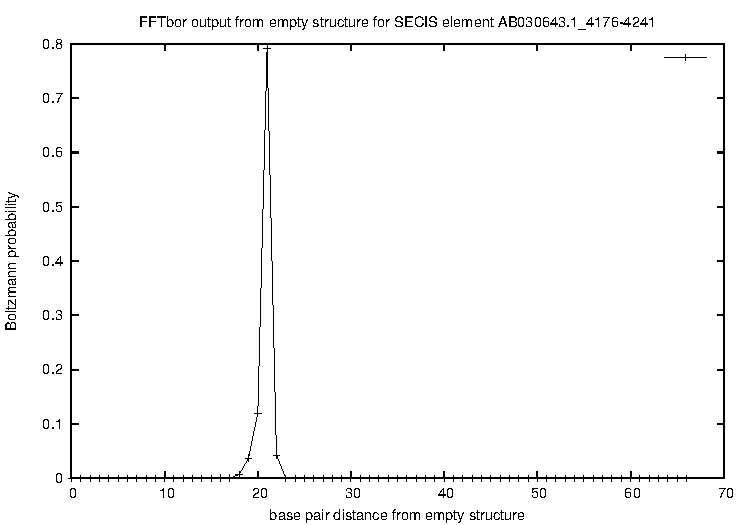
\includegraphics[width=.3\textwidth]{Figures/FFTbor/AB030643_1_4176-4241.pdf}
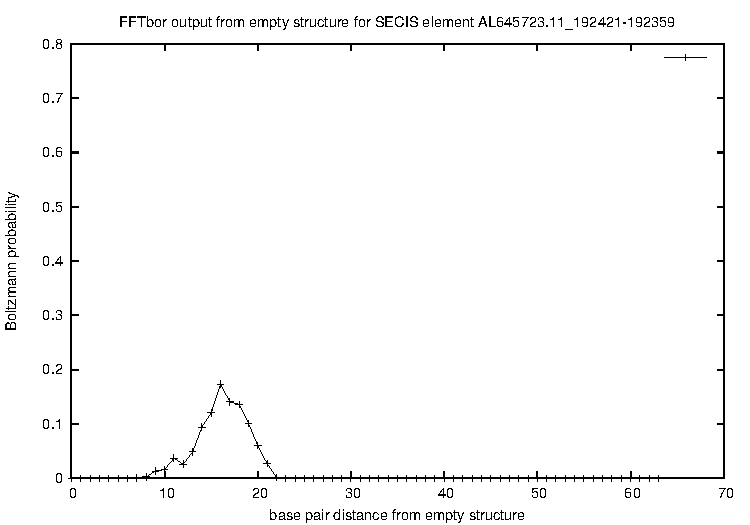
\includegraphics[width=.3\textwidth]{Figures/FFTbor/AL645723_11_192421-192359.pdf}
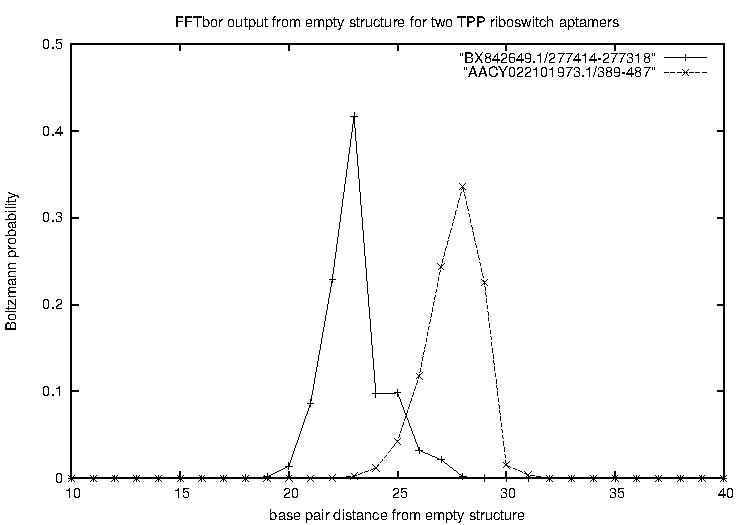
\includegraphics[width=.3\textwidth]{Figures/FFTbor/FFTborOutputFromEmptyStrForTPPriboswitches.pdf}
\caption[Example of the graphical output of \fftbor, when the empty structure is chosen as initial structure \strSt]{This figure represents the
graphical output of \fftbor, when the empty structure is chosen as
initial structure \strSt.
The $x$-axis represents the number of base pairs per structure,
taken over the ensemble of all secondary structures for the given RNA
sequence; the $y$-axis represents Boltzmann probability
$p(k) = \sfrac{\bfZ{k}{}}{\fullZ}$,
where \fullZ is the partition function for all secondary structures
having exactly $k$ base pairs.
{\em (Left)}
For the selenocysteine (SECIS) element AB$030643.1$/$4176$--$4241$ from Rfam family
RF$00031$, the standard deviation $\sigma$ of the number of base pairs,
taken over the ensemble of all secondary structures, is
$0.7276$, while the logarithm base $10$ of the \mfpt ($\log_{10}(\text{MFPT})$)
is $4.75$.
{\em (Center)}
For the selenocysteine (SECIS) element
AL$645723.11$/$192421$--$192359$ from Rfam family
RF$00031$, the standard deviation $\sigma$ of the number of base pairs,
taken over the ensemble of all secondary structures, is
$2.6794$, while $\log_{10}(\text{MFPT})$ is $5.69$.
Among the $61$ sequences in the seed alignment of RF$00031$,
AB$030643.1$/$4176$--$4241$ was the fastest folder, while
AL$645723.11$/$192421$--$192359$ was the slowest folder.
{\em (Right)}
Superimposition of output of \fftbor for two TPP \rb aptamers: the
$97$ nt sequence BX$842649.1$/$277414$--$277318$ and the
$99$ nt sequence AACY$022101973.1$/$389$--$487$, both obtained when
taking the empty structure for the initial structure \strSt.
The mean $\mu$ for the \fftbor structural profile near the empty
structure is $23.0203$  [resp. $27.5821$], the
standard deviation $\sigma$ for the \fftbor structural profile
is $2.2253$  [resp. $1.9857$], and the \kinfold MFPT is
$311,075.06$ [resp. $61,575.69$] for the TPP \rb aptamer
AB$030643.1$/$4176$--$4241$ [resp. AL$645723.11$/$192421$--$192359$].
The right panel of this figure should be compared with Figure
\ref{fig:fftbor:tppDistributions}.
These anecdotal results bear up the correlation between standard deviation
$\sigma$ and $\log_{10}(\text{MFPT})$ described in Table \ref{table:correlationFFTborEmpty}.
}
\label{fig:fftbor:correlationFFTborEmpty}
\end{figure}

In the right panel of \Figref{fftbor:correlationFFTborEmpty}, we
applied \fftbor to each of the two randomly chosen TPP \rb
aptamers BX$842649.1$/$277414$--$277318$ and AACY$022101973.1$/$389$--$487$, starting
from the empty reference structure $\strSt=\varnothing$.
The mean for the \fftbor structural profile near the empty
structure is $\mu_1=23.0203$  [resp. $\mu_2=27.5821$], the
standard deviation $\sigma$ for the \fftbor structural profile
is $\sigma_1=2.2253$  [resp. $\sigma_2=1.9857$], and the \kinfold MFPT is
$311,075.06$ [resp. $61,575.69$] for the TPP \rb aptamer
AB$030643.1$/$4176$--$4241$ [resp.  AL$645723.11$/$192421$--$192359$]. This anecdotal evidence supports the hypothesis that small standard deviation in \fftbor distribution is correlated with fast folding.

Additionally, we randomized the TPP \rbs BX$842649.1$/$277414$--$277318$ and AACY$022101973.1$/$389$--$487$ by using our implementation of the Altschul-Erikson dinucleotide shuffle algorithm
\citep{altschulErikson:dinucleotideShuffle}, and then applied \fftbor to these
sequences, starting from the empty structure.  The mean $\mu_1$ and standard
deviation $\sigma_1$ for the \fftbor distribution for randomized BX$842649$ are
respectively $\mu_1=19.93$ and $\sigma_1=2.88$, while those for randomized
AACY$022101973$ are $\mu_2=24.39$ and $\sigma_2=24.00$. Running \kinfold, with a
maximum of $500,000$ steps with $30$ replicates (as explained in the text), we
found
that for randomized BX$842649$, all $30$ runs converged yielding a \mfpt
(MFPT) of $13,022.58$ with standard deviation of $15,221.78$. In contrast for
randomized AACY$022101973$, only $15$ out of $30$ runs converged within $500,000$ steps,
and discounting these nonconvergent data, we obtain an average \mfpt
(MFPT) of $94,446.93$ with standard deviation of $157,107.43$. This additional
test provides more anecdotal evidence supporting our hypothesis that small
standard deviation $\sigma$ in \fftbor probability density is correlated with fast folding, as measured by MFPT.

This notion of correlation between the coarse-grained energy landscape and
kinetics is what motivates the work described in Chapters \ref{ch:ffttwo}
and \ref{ch:hermes}, where a more detailed explanation of kinetics is provided,
and additional evidence is provided to support this claim.

\section{Performance characteristics of \fftbor and \rnabor}
\label{sec:fftbor:speed}

As visible from the defining recursions, the algorithmic time complexity of
\rnabor is \On{5} and space complexity is \On{3}, where $n$ is
the length of input RNA sequence. In contrast, the time complexity of
\fftbor is \On{4} and space complexity is \On{2}.
While \fftbor saves an order of magnitude in performance and memory,
\rnabor has the benefit of producing suboptimal structures $\text{MFE}_k$
for all $0 \leq k \leq n$, whose free energy is minimal across all structures
having \bpd $k$ from input structures \strSt.
\Figref{fftbor:benchmarking} displays run time curves for both
\rnabor and \fftbor, when the initial structure \strSt is
taken to be either the empty structure or the \mfe
(MFE) structure.

Here, we compare the run time of \rnabor \citep{freyhult.b07} and
the (unparallelized version of) \fftbor, using
a Dell Power Edge $1950$, $2$ x Intel Xeon E$5430$ Quad
core with $2.80$ GHz and $16$ GB RAM. For $n = 20,40,60,\dots,300$, in step
size of $20$ nt, we generated $n$ random RNA sequences of length $n$ with equal
probability for each nucleotide A,C,G,U (i.e. a 0th order Markov chain).
For values of $n \leq 200$, $100$ random sequences of length
$n$ were generated, while for values of $220 \leq n \leq 300$, only
$10$ sequences of length $n$ were generated.
RNA sequences larger than $300$ nt were not tested,
due to \On{3} memory constraints required by \rnabor.
For each RNA sequence, \rnabor and \fftbor were both run,
each starting with empty initial structure \strSt, and also
with initial sequence \strSt taken to be the MFE structure.
Each data point in the table comprises the average run time for three
independent evaluations.

\begin{figure}[!ht]
\centering
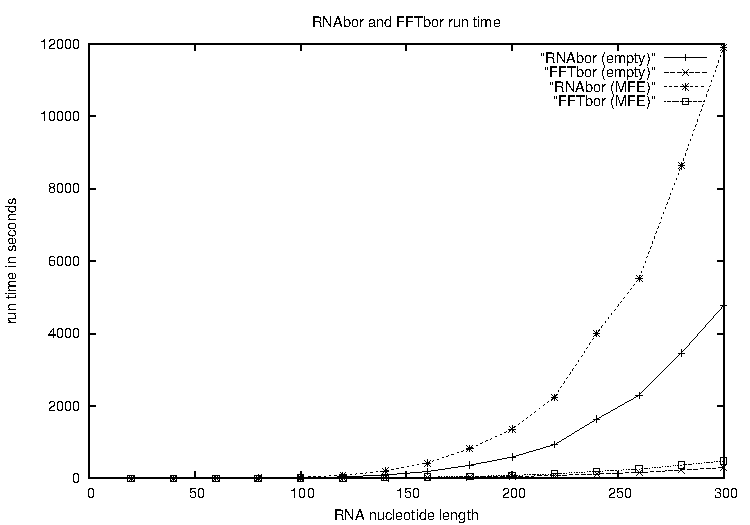
\includegraphics[width=.9\textwidth]{Figures/FFTbor/rnaborfftborRunTimeEvan.pdf}
\caption[Run times in seconds for \rnabor and \fftbor, on random RNA
of length $20,\dots,300$ in step size of $20$ nt]{Run times in seconds for \rnabor and \fftbor, on random RNA
of length $20,40,60,\dots,300$ in step size of $20$ nt. Each algorithm
was run with the empty initial structure \strSt, see rows
\rnabor (empty), \fftbor (empty), and with the \mfes as the initial structure
\strSt, see rows
\rnabor (MFE) and \fftbor (MFE). Note that for both \rnabor
and \fftbor, the run time increases when \strSt is the MFE structure,
rather than the empty structure. Notice the radical improvement in the
run time of \fftbor over that of \rnabor.
}
\label{fig:fftbor:benchmarking}
\end{figure}

\subsection{OpenMP parallelization of \fftbor}
\label{subsec:fftbor:openmp}

OpenMP is a simple and flexible
multi-platform shared-memory parallel programming environment, that supports
parallelizations of C/C++ code---see \url{http://openmp.org/}.
Using OpenMP primitives, we created multiple threads to evaluate the polynomial
\fullZx on different \nRoUs. \Figref{fftbor:benchmarkingParallel}
presents benchmarks, executed on
a $24$-core AMD Opteron $6172$ with $2.10$GHz and $64$GB RAM, for the speedup
of \fftbor as a function of the number of cores.
The data in Table \ref{table:fftborBenchmarkingParallel} describes average
run time in seconds ($\pm$ one standard deviation) for running \fftbor
on random RNA of length $200,250,300,400,450,500$ with either $1$ or $2$ cores.
\Figref{fftbor:benchmarkingParallel}
presents similar data for running
\fftbor on $2,3,6,4,12,15,20$ cores.

\begin{table}[!ht]
\centering
\begin{tabularx}{\linewidth}{c *{2}{R}}
\toprule
\small{$n$} & \small{Single core} & \small{Two cores} \\
\cmidrule(lr){1-3}
$200$ & $123.2 \pm 16.2$ & $61.8 \pm 8.0$ \\
$250$ & $331.1 \pm 27.2$ & $166.1 \pm 13.7$ \\
$300$ & $723.4 \pm 59.9$ & $365.2 \pm 30.1$ \\
$350$ & $1,380.8 \pm 95.2$ & $698.4 \pm 46.9$ \\
$400$ & $2,239.1 \pm 210.9$ & $1,129.5 \pm 104.3$ \\
$450$ & $3,635.0 \pm 857.4$ & $1,980.9 \pm 126.5$ \\
$500$ & $5,076.7 \pm 1,292.1$ & $3,389.8 \pm 788.4$ \\
\bottomrule
\end{tabularx}
\caption[Table showing parallel run times in seconds
for \fftbor, using OpenMP]{Table showing parallel run times in seconds
for \fftbor, using OpenMP---\url{http://openmp.org/}.
For each sequence length $200,\dots,500$,
five random RNAs were generated using equal probability for each nucleotide
A,C,G,U. Run time in seconds, plus or minus one standard deviation, are
given for a $24$-core
AMD Opteron $6172$ running at $2.10$GHz with $64$GB RAM, with only $1$ [resp. $2$] cores
used.}
\label{table:fftborBenchmarkingParallel}
\end{table}

\begin{figure}[!ht]
\centering
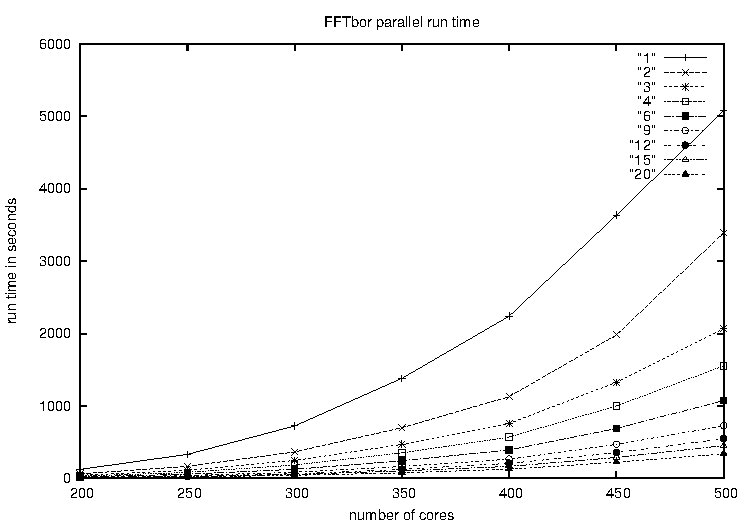
\includegraphics[width=.75\textwidth]{Figures/FFTbor/fftborParallelRunTimes.pdf}
\caption[]{Graph showing parallel run time of \fftbor as a function of
sequence length, running on an AMD Opteron $6172$ running at $2.10$GHz with $64$GB RAM,
using respectively $1,2,3,4,6,9,12,15,20$ cores.
}
\label{fig:fftbor:benchmarkingParallel}
\end{figure}
